\documentclass{article}

% content/resources/templates/preamble.tex
\usepackage[margin=0.6in]{geometry}
\author{Milav Dabgar}
\usepackage{amsmath,amssymb,amsthm}
\usepackage{booktabs}
\usepackage{multirow}
\usepackage{xcolor}
\usepackage{tcolorbox}
\tcbuselibrary{breakable,skins}
\usepackage[colorlinks=true,linkcolor=blue]{hyperref}
\usepackage{titlesec}
\usepackage{enumitem}
\usepackage{tikz}
\usepackage{pgfplots}
\usepackage{circuitikz}
\usepackage[version=4]{mhchem}
\usepackage{longtable}
\usepackage{array}
\usepackage{float}
\usepackage{caption}
\usepackage{listings}

\lstset{
  basicstyle=\small\ttfamily,
  breaklines=true,
  breakatwhitespace=false,
  postbreak=\mbox{\textcolor{red}{$\hookrightarrow$}\space},
  float=false,
  numbers=left,
  numberstyle=\tiny\color{gray},
  numbersep=10pt,
  xleftmargin=2em,
  keywordstyle=\color{blue},
  commentstyle=\color{green!60!black},
  stringstyle=\color{purple},
  backgroundcolor=\color{gray!5},
  showstringspaces=false,
  tabsize=2,
  captionpos=b,
  keepspaces=true,
  columns=flexible
}

\pgfplotsset{compat=1.18}
\usetikzlibrary{shapes,arrows,positioning,calc,patterns,decorations.pathmorphing,decorations.markings,arrows.meta}

% Color scheme
\definecolor{headcolor}{RGB}{0,102,204}
\definecolor{keycolor}{RGB}{220,20,60}
\definecolor{solutioncolor}{RGB}{34,139,34}
\definecolor{mnemoniccolor}{RGB}{148,0,211}
\definecolor{codecolor}{RGB}{0,0,100}

% Spacing
\setlength{\parskip}{3pt}
\setlist[itemize]{nosep}
\setlist[enumerate]{nosep}

% Title formatting
\titleformat{\section}{\Large\bfseries\color{headcolor}}{\thesection}{1em}{}
\titleformat{\subsection}{\large\bfseries\color{headcolor}}{\thesubsection}{1em}{}

% Pandoc tightlist compatibility
\providecommand{\tightlist}{%
  \setlength{\itemsep}{0pt}\setlength{\parskip}{0pt}}

% Pandoc longtable compatibility
\newcounter{none}
\def\thenone{}


% content/resources/templates/english-boxes.tex
% This file is currently empty - it exists to maintain consistency with the import structure.
% Add custom environments here if needed in the future.


% Custom commands for GTU solutions
% This file defines semantic commands for consistent formatting

% Question command with automatic formatting
\newcommand{\question}[2]{%
  \section*{Question #1}%
  \textbf{#2}%
}

% OR question variant
\newcommand{\questionor}[2]{%
  \section*{Question #1 OR}%
  \textbf{#2}%
}

% Proper table environment with caption
\newenvironment{answertable}[1]{%
  \begin{table}[htbp]
  \centering
  \caption{#1}
}{%
  \end{table}
}

% Proper figure environment for diagrams
\newenvironment{answerdiagram}[1]{%
  \begin{figure}[htbp]
  \centering
  \caption{#1}
}{%
  \end{figure}
}

% Semantic markup for key terms
\newcommand{\keyword}[1]{\textbf{#1}}
\newcommand{\code}[1]{\texttt{#1}}
\newcommand{\classname}[1]{\texttt{#1}}
\newcommand{\methodname}[1]{\texttt{#1}}

% Proper quotation marks
\newcommand{\mnemonic}[1]{``#1''}


\title{Digital \& Data Communication (4343201) - Summer 2025 Solution}
\date{May 15, 2025}

\begin{document}
\maketitle

\questionmarks{1(a)}{3}{Define bit rate, baud rate and bandwidth}

\begin{solutionbox}
\begin{center}
\captionof{table}{Definition of Communication Parameters}
\begin{tabulary}{\linewidth}{|L|L|L|}
\hline
\textbf{Parameter} & \textbf{Definition} & \textbf{Unit} \\ \hline
\textbf{Bit Rate} & Number of bits transmitted per second & bps (bits per second) \\ \hline
\textbf{Baud Rate} & Number of signal changes per second & Baud \\ \hline
\textbf{Bandwidth} & Range of frequencies in communication channel & Hz (Hertz) \\ \hline
\end{tabulary}
\end{center}

\begin{itemize}
    \item \keyword{Bit rate}: Actual data transmission speed
    \item \keyword{Baud rate}: Modulation rate or symbol rate
    \item \keyword{Bandwidth}: Channel capacity for frequency range
\end{itemize}
\end{solutionbox}

\begin{mnemonicbox}
\mnemonic{Bits Baud Bandwidth - BBB for communication}
\end{mnemonicbox}

\questionmarks{1(b)}{4}{Explain TDM with block diagram}

\begin{solutionbox}
\begin{center}
\begin{tikzpicture}[node distance=1.5cm, auto]
    \node [gtu block] (mux) {Time Division Multiplexer};
    \node [gtu block, right=3cm of mux] (demux) {Time Division Demultiplexer};
    
    \node [left=1cm of mux] (in2) {Input 2};
    \node [above=0.5cm of in2] (in1) {Input 1};
    \node [below=0.5cm of in2] (in3) {Input 3};
    \node [below=0.5cm of in2] (in4) {Input 4};
    
    \node [right=1cm of demux] (out2) {Output 2};
    \node [above=0.5cm of out2] (out1) {Output 1};
    \node [below=0.5cm of out2] (out3) {Output 3};
    \node [below=0.5cm of out2] (out4) {Output 4};
    
    \draw [gtu arrow] (in1) -- (mux.west |- in1);
    \draw [gtu arrow] (in2) -- (mux.west |- in2);
    \draw [gtu arrow] (in3) -- (mux.west |- in3);
    \draw [gtu arrow] (in4) -- (mux.west |- in4);
    
    \draw [gtu arrow] (mux) -- node {Transmission Channel} (demux);
    
    \draw [gtu arrow] (demux.east |- out1) -- (out1);
    \draw [gtu arrow] (demux.east |- out2) -- (out2);
    \draw [gtu arrow] (demux.east |- out3) -- (out3);
    \draw [gtu arrow] (demux.east |- out4) -- (out4);
\end{tikzpicture}
\captionof{figure}{Time Division Multiplexing (TDM)}
\end{center}

\begin{itemize}
    \item \keyword{TDM principle}: Multiple signals share single channel by time slots
    \item \keyword{Time slots}: Each input gets dedicated time period
    \item \keyword{Synchronization}: Transmitter and receiver must be synchronized
    \item \keyword{Applications}: Digital telephone systems, computer networks
\end{itemize}
\end{solutionbox}

\begin{mnemonicbox}
\mnemonic{Time Divided Multiple - TDM shares time}
\end{mnemonicbox}

\questionmarks{1(c)}{7}{Explain block diagram of digital communication system}

\begin{solutionbox}
\begin{center}
\begin{tikzpicture}[node distance=1.2cm, auto, font=\small]
    \node [gtu block] (source) {Information Source};
    \node [gtu block, right=0.8cm of source] (senc) {Source Encoder};
    \node [gtu block, right=0.8cm of senc] (cenc) {Channel Encoder};
    \node [gtu block, right=0.8cm of cenc] (mod) {Digital Modulator};
    
    % New row for return path to save width
    \node [gtu block, below=1.5cm of mod] (channel) {Channel};
    \node [gtu block, below=1.5cm of channel] (demod) {Digital Demodulator};
    \node [gtu block, left=0.8cm of demod] (cdec) {Channel Decoder};
    \node [gtu block, left=0.8cm of cdec] (sdec) {Source Decoder};
    \node [gtu block, left=0.8cm of sdec] (dest) {Destination};
    
    \node [above=0.8cm of channel] (noise) {Noise};

    \draw [gtu arrow] (source) -- (senc);
    \draw [gtu arrow] (senc) -- (cenc);
    \draw [gtu arrow] (cenc) -- (mod);
    \draw [gtu arrow] (mod) -- (channel);
    \draw [gtu arrow] (channel) -- (demod);
    \draw [gtu arrow] (demod) -- (cdec);
    \draw [gtu arrow] (cdec) -- (sdec);
    \draw [gtu arrow] (sdec) -- (dest);
    \draw [gtu arrow] (noise) -- (channel);
\end{tikzpicture}
\captionof{figure}{Digital Communication System}
\end{center}

\begin{center}
\captionof{table}{System Components}
\begin{tabulary}{\linewidth}{|L|L|}
\hline
\textbf{Component} & \textbf{Function} \\ \hline
\textbf{Source Encoder} & Converts analog to digital \\ \hline
\textbf{Channel Encoder} & Adds error correction codes \\ \hline
\textbf{Digital Modulator} & Converts digital to analog signal \\ \hline
\textbf{Channel} & Transmission medium \\ \hline
\textbf{Digital Demodulator} & Recovers digital signal \\ \hline
\textbf{Channel Decoder} & Detects and corrects errors \\ \hline
\textbf{Source Decoder} & Reconstructs original signal \\ \hline
\end{tabulary}
\end{center}

\begin{itemize}
    \item \keyword{Advantages}: Noise immunity, error correction capability
    \item \keyword{Processing}: Digital signal processing techniques
    \item \keyword{Reliability}: Better performance over long distances
\end{itemize}
\end{solutionbox}

\begin{mnemonicbox}
\mnemonic{Source Channel Modulate Transmit Demodulate Decode - SCMTDD}
\end{mnemonicbox}

\questionmarks{1(c OR)}{7}{Explain different types of Communication channel}

\begin{solutionbox}
\begin{center}
\captionof{table}{Channel Types}
\begin{tabulary}{\linewidth}{|L|L|L|}
\hline
\textbf{Channel Type} & \textbf{Characteristics} & \textbf{Applications} \\ \hline
\textbf{Telephone Channel} & 300-3400 Hz bandwidth & Voice communication \\ \hline
\textbf{Coaxial Cable} & High bandwidth, shielded & Cable TV, Internet \\ \hline
\textbf{Optical Fiber} & Very high bandwidth, light signals & Long distance, high speed \\ \hline
\textbf{Wireless Channel} & Radio frequency transmission & Mobile, satellite \\ \hline
\textbf{Satellite Channel} & Long distance, space communication & Global communication \\ \hline
\end{tabulary}
\end{center}

\begin{itemize}
    \item \keyword{Bandwidth}: Different channels offer varying frequency ranges
    \item \keyword{Noise characteristics}: Each channel has specific noise properties
    \item \keyword{Distance capability}: Varies from local to global coverage
    \item \keyword{Cost factors}: Installation and maintenance costs differ
\end{itemize}
\end{solutionbox}

\begin{mnemonicbox}
\mnemonic{Telephone Coax Optical Wireless Satellite - TCOWS channels}
\end{mnemonicbox}

\questionmarks{2(a)}{3}{Draw the modulation waveform for ASK, FSK and BPSK for the digital sequence 11100110}

\begin{solutionbox}
\begin{center}
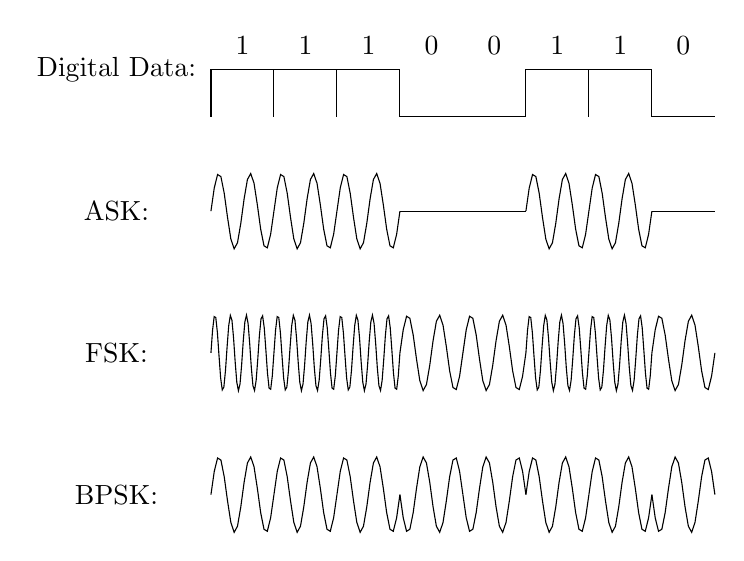
\begin{tikzpicture}[x=0.8cm,y=0.6cm]
    % Digital Data
    \node at (-1.5, 1) {Digital Data:};
    \foreach \x/\val in {0/1, 1/1, 2/1, 3/0, 4/0, 5/1, 6/1, 7/0} {
        \draw (\x,0) -- (\x,\val) -- (\x+1,\val) -- (\x+1,0); 
        \node at (\x+0.5, 1.5) {\val};
    }
    
    % ASK
    \node at (-1.5, -2) {ASK:};
    \foreach \x/\val in {0/1, 1/1, 2/1, 3/0, 4/0, 5/1, 6/1, 7/0} {
        \ifnum\val=1
            \draw[domain=\x:\x+1, samples=20] plot (\x, {sin(360*(\x)*2) * 0.8 - 2});
        \else
            \draw (\x,-2) -- (\x+1,-2);
        \fi
    }
    
    % FSK
    \node at (-1.5, -5) {FSK:};
    \foreach \x/\val in {0/1, 1/1, 2/1, 3/0, 4/0, 5/1, 6/1, 7/0} {
        \ifnum\val=1
            % High freq
            \draw[domain=\x:\x+1, samples=40] plot (\x, {sin(360*(\x)*4) * 0.8 - 5});
        \else
            % Low freq
            \draw[domain=\x:\x+1, samples=20] plot (\x, {sin(360*(\x)*2) * 0.8 - 5});
        \fi
    }
    
    % BPSK
    \node at (-1.5, -8) {BPSK:};
    \foreach \x/\val in {0/1, 1/1, 2/1, 3/0, 4/0, 5/1, 6/1, 7/0} {
        \ifnum\val=1
            % 0 phase
            \draw[domain=\x:\x+1, samples=20] plot (\x, {sin(360*(\x)*2) * 0.8 - 8});
        \else
            % 180 phase
            \draw[domain=\x:\x+1, samples=20] plot (\x, {-sin(360*(\x)*2) * 0.8 - 8});
        \fi
    }
\end{tikzpicture}
\captionof{figure}{Modulation Waveforms}
\end{center}

\begin{itemize}
    \item \keyword{ASK}: Amplitude Shift Keying
    \item \keyword{FSK}: Frequency Shift Keying
    \item \keyword{BPSK}: Binary Phase Shift Keying
\end{itemize}
\end{solutionbox}

\begin{mnemonicbox}
\mnemonic{ASK Amplitude, FSK Frequency, BPSK Phase - AFP modulation}
\end{mnemonicbox}

\questionmarks{2(b)}{4}{Explain the basic principle and generation of frequency shift keying (FSK) signal}

\begin{solutionbox}
\begin{center}
\captionof{table}{FSK Generation}
\begin{tabulary}{\linewidth}{|L|L|L|}
\hline
\textbf{Binary Data} & \textbf{Frequency} & \textbf{Output} \\ \hline
Logic `1' & $f_1$ (High frequency) & High freq carrier \\ \hline
Logic `0' & $f_0$ (Low frequency) & Low freq carrier \\ \hline
\end{tabulary}
\end{center}

\begin{center}
\begin{tikzpicture}[node distance=1.5cm, auto]
    \node [gtu block] (sel) {Frequency Selector};
    \node [gtu block, left=1.5cm of sel, yshift=1cm] (osc1) {Oscillator 1 ($f_1$)};
    \node [gtu block, left=1.5cm of sel, yshift=-1cm] (osc2) {Oscillator 2 ($f_0$)};
    \node [left=1.5cm of sel] (data) {Digital Data};
    \node [right=1.5cm of sel] (out) {FSK Output};
    
    \draw [gtu arrow] (osc1) -| (sel);
    \draw [gtu arrow] (osc2) -| (sel);
    \draw [gtu arrow] (data) -- (sel);
    \draw [gtu arrow] (sel) -- (out);
\end{tikzpicture}
\captionof{figure}{FSK Generation}
\end{center}

\begin{itemize}
    \item \keyword{Principle}: Binary data controls carrier frequency
    \item \keyword{Two frequencies}: $f_1$ for `1' and $f_0$ for `0'
    \item \keyword{Constant amplitude}: Only frequency changes
    \item \keyword{Detection}: Frequency discrimination at receiver
\end{itemize}
\end{solutionbox}

\begin{mnemonicbox}
\mnemonic{Frequency Shifts Key - FSK frequency control}
\end{mnemonicbox}

\questionmarks{2(c)}{7}{Explain the working of QPSK modulator and Demodulator with block diagram and constellation diagram}

\begin{solutionbox}
\textbf{QPSK Modulator:}
\begin{center}
\begin{tikzpicture}[node distance=1.5cm, auto]
    \node [gtu block] (sp) {Serial to Parallel};
    \node [gtu block, right=2cm of sp, yshift=1cm] (mult1) {Multiplier 1};
    \node [gtu block, right=2cm of sp, yshift=-1cm] (mult2) {Multiplier 2};
    \node [gtu block, right=2cm of mult1, yshift=-1cm] (adder) {Adder};
    
    \node [left=1cm of sp] (input) {Serial Data};
    \node [above=1cm of mult1] (car1) {Carrier $\cos(\omega t)$};
    \node [below=1cm of mult2] (car2) {Carrier $\sin(\omega t)$};
    \node [right=1cm of adder] (out) {QPSK Output};
    
    \draw [gtu arrow] (input) -- (sp);
    \draw [gtu arrow] (sp) -- node[above, sloped] {I Channel} (mult1);
    \draw [gtu arrow] (sp) -- node[below, sloped] {Q Channel} (mult2);
    \draw [gtu arrow] (car1) -- (mult1);
    \draw [gtu arrow] (car2) -- (mult2);
    \draw [gtu arrow] (mult1) -| (adder);
    \draw [gtu arrow] (mult2) -| (adder);
    \draw [gtu arrow] (adder) -- (out);
\end{tikzpicture}
\captionof{figure}{QPSK Modulator Block Diagram}
\end{center}

\textbf{Constellation Diagram:}
\begin{center}
\begin{tikzpicture}[scale=1.5]
    \draw[->] (-2,0) -- (2,0) node[right] {I};
    \draw[->] (0,-2) -- (0,2) node[above] {Q};
    
    \foreach \x/\y/\l in {1/1/00 (45$^\circ$), -1/1/01 (135$^\circ$), -1/-1/11 (225$^\circ$), 1/-1/10 (315$^\circ$)} {
        \draw[fill] (\x,\y) circle (2pt);
        \node at (\x*1.4, \y*1.4) {\l};
        \draw[dashed] (0,0) -- (\x,\y);
    }
\end{tikzpicture}
\captionof{figure}{QPSK Constellation Diagram}
\end{center}

\begin{center}
\captionof{table}{QPSK Truth Table}
\begin{tabulary}{\linewidth}{|C|C|C|C|}
\hline
\textbf{I} & \textbf{Q} & \textbf{Phase} & \textbf{Symbol} \\ \hline
0 & 0 & 45$^\circ$ & 00 \\ \hline
0 & 1 & 135$^\circ$ & 01 \\ \hline
1 & 1 & 225$^\circ$ & 11 \\ \hline
1 & 0 & 315$^\circ$ & 10 \\ \hline
\end{tabulary}
\end{center}

\begin{itemize}
    \item \keyword{Four phases}: 45$^\circ$, 135$^\circ$, 225$^\circ$, 315$^\circ$
    \item \keyword{Two bits per symbol}: Higher data rate
    \item \keyword{Constant envelope}: Amplitude remains constant
    \item \keyword{Demodulation}: Phase detection and parallel to serial conversion
\end{itemize}
\end{solutionbox}

\begin{mnemonicbox}
\mnemonic{Quadrature Phase Shift Key - QPSK four phases}
\end{mnemonicbox}

\questionmarks{2(a OR)}{3}{Draw the block diagram of ASK modulator and describe working of it}

\begin{solutionbox}
\begin{center}
\begin{tikzpicture}[node distance=1.5cm, auto]
    \node [gtu block] (switch) {Switch/Multiplier};
    \node [left=1.5cm of switch] (data) {Digital Data};
    \node [above=1cm of switch] (carrier) {Carrier Oscillator};
    \node [right=1.5cm of switch] (out) {ASK Output};
    
    \draw [gtu arrow] (data) -- (switch);
    \draw [gtu arrow] (carrier) -- (switch);
    \draw [gtu arrow] (switch) -- (out);
\end{tikzpicture}
\captionof{figure}{ASK Modulator}
\end{center}

\begin{itemize}
    \item \keyword{Working principle}: Digital data controls carrier amplitude
    \item \keyword{Logic `1'}: Carrier transmitted with full amplitude
    \item \keyword{Logic `0'}: No carrier transmitted (zero amplitude)
    \item \keyword{Simple implementation}: Uses analog switch or multiplier
\end{itemize}
\end{solutionbox}

\begin{mnemonicbox}
\mnemonic{Amplitude Shift Key - ASK amplitude control}
\end{mnemonicbox}

\questionmarks{2(b OR)}{4}{Explain the principal of 16-QAM and draw the constellation diagram}

\begin{solutionbox}
\textbf{16-QAM Constellation:}
\begin{center}
\begin{tikzpicture}[scale=1.2]
    \draw[->] (-3,0) -- (3,0) node[right] {I};
    \draw[->] (0,-3) -- (0,3) node[above] {Q};
    
    \foreach \x in {-1.5, -0.5, 0.5, 1.5} {
        \foreach \y in {-1.5, -0.5, 0.5, 1.5} {
            \draw[fill] (\x,\y) circle (2pt);
        }
    }
\end{tikzpicture}
\captionof{figure}{16-QAM Constellation}
\end{center}

\begin{center}
\captionof{table}{16-QAM Characteristics}
\begin{tabulary}{\linewidth}{|L|L|}
\hline
\textbf{Parameter} & \textbf{Value} \\ \hline
\textbf{Bits per symbol} & 4 bits \\ \hline
\textbf{Number of states} & 16 \\ \hline
\textbf{Amplitude levels} & 4 levels \\ \hline
\textbf{Phase levels} & 4 phases \\ \hline
\end{tabulary}
\end{center}

\begin{itemize}
    \item \keyword{Principle}: Combines amplitude and phase modulation
    \item \keyword{Higher data rate}: 4 bits per symbol
    \item \keyword{Complex modulation}: Requires precise amplitude and phase control
    \item \keyword{Applications}: High-speed digital communication
\end{itemize}
\end{solutionbox}

\begin{mnemonicbox}
\mnemonic{16 Quadrature Amplitude Modulation - 16QAM complex signals}
\end{mnemonicbox}

\questionmarks{2(c OR)}{7}{Explain working of BPSK modulator and demodulator with block diagram and waveform}

\begin{solutionbox}
\textbf{BPSK Modulator:}
\begin{center}
\begin{tikzpicture}[node distance=1.5cm, auto]
    \node [gtu block] (nrz) {NRZ Encoder};
    \node [gtu block, right=1.5cm of nrz] (mod) {Balanced Modulator};
    \node [above=1cm of mod] (osc) {Carrier Oscillator};
    \node [left=1.5cm of nrz] (in) {Digital Data};
    \node [right=1.5cm of mod] (out) {BPSK Output};
    
    \draw [gtu arrow] (in) -- (nrz);
    \draw [gtu arrow] (nrz) -- (mod);
    \draw [gtu arrow] (osc) -- (mod);
    \draw [gtu arrow] (mod) -- (out);
\end{tikzpicture}
\captionof{figure}{BPSK Modulator}
\end{center}

\textbf{BPSK Demodulator:}
\begin{center}
\begin{tikzpicture}[node distance=1.5cm, auto]
    \node [gtu block] (demod) {Balanced Demodulator};
    \node [gtu block, right=1.5cm of demod] (lpf) {Low Pass Filter};
    \node [gtu block, right=1.5cm of lpf] (dec) {Decision Circuit};
    \node [above=1cm of demod] (local) {Local Carrier};
    \node [left=1.5cm of demod] (in) {BPSK Input};
    \node [right=1.5cm of dec] (out) {Digital Output};
    
    \draw [gtu arrow] (in) -- (demod);
    \draw [gtu arrow] (local) -- (demod);
    \draw [gtu arrow] (demod) -- (lpf);
    \draw [gtu arrow] (lpf) -- (dec);
    \draw [gtu arrow] (dec) -- (out);
\end{tikzpicture}
\captionof{figure}{BPSK Demodulator}
\end{center}

\textbf{Waveforms:}
\begin{center}
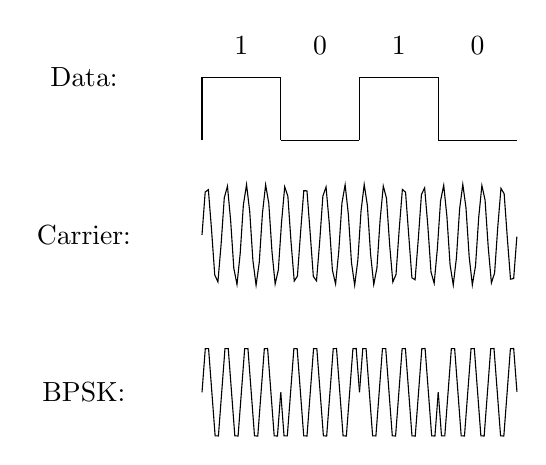
\begin{tikzpicture}[x=1cm,y=0.8cm]
    % Data
    \node at (-1.5, 1) {Data:};
    \foreach \x/\val in {0/1, 1/0, 2/1, 3/0} {
        \draw (\x,0) -- (\x,\val) -- (\x+1,\val) -- (\x+1,0);
        \node at (\x+0.5, 1.5) {\val};
    }
    
    % Carrier
    \node at (-1.5, -1.5) {Carrier:};
    \draw[domain=0:4, samples=100] plot (\x, {sin(360*\x*4) * 0.8 - 1.5});
    
    % BPSK
    \node at (-1.5, -4) {BPSK:};
    \foreach \x/\val in {0/1, 1/0, 2/1, 3/0} {
        \ifnum\val=1
            \draw[domain=\x:\x+1, samples=25] plot (\x, {sin(360*\x*4) * 0.8 - 4});
        \else
            \draw[domain=\x:\x+1, samples=25] plot (\x, {-sin(360*\x*4) * 0.8 - 4});
        \fi
    }
\end{tikzpicture}
\captionof{figure}{BPSK Waveforms}
\end{center}

\begin{itemize}
    \item \keyword{Phase shift}: 180$^\circ$ between `1' and `0'
    \item \keyword{Coherent detection}: Requires synchronized carrier
    \item \keyword{Best performance}: Lowest bit error rate
    \item \keyword{Constant envelope}: Amplitude remains constant
\end{itemize}
\end{solutionbox}

\begin{mnemonicbox}
\mnemonic{Binary Phase Shift Key - BPSK two phases}
\end{mnemonicbox}

\questionmarks{3(a)}{3}{Define Channel Capacity in terms of SNR and explain importance of it}

\begin{solutionbox}
\textbf{Shannon's Channel Capacity Formula:}
\begin{center}
\captionof{table}{Channel Capacity Formula}
\begin{tabulary}{\linewidth}{|L|L|}
\hline
\textbf{Formula} & $C = B \log_2(1 + S/N)$ \\ \hline
\textbf{C} & Channel capacity (bps) \\ \hline
\textbf{B} & Bandwidth (Hz) \\ \hline
\textbf{S/N} & Signal-to-Noise ratio \\ \hline
\end{tabulary}
\end{center}

\begin{itemize}
    \item \keyword{Importance}: Maximum theoretical data rate
    \item \keyword{SNR effect}: Higher SNR allows higher capacity
    \item \keyword{Bandwidth trade-off}: Can exchange bandwidth for SNR
    \item \keyword{Design limit}: Sets upper bound for system design
\end{itemize}
\end{solutionbox}

\begin{mnemonicbox}
\mnemonic{Channel Capacity Shannon's Limit - CCSL}
\end{mnemonicbox}

\questionmarks{3(b)}{4}{Describe Asynchronous and synchronous serial data communication techniques}

\begin{solutionbox}
\begin{center}
\captionof{table}{Synchronous vs Asynchronous}
\begin{tabulary}{\linewidth}{|L|L|L|}
\hline
\textbf{Parameter} & \textbf{Synchronous} & \textbf{Asynchronous} \\ \hline
\textbf{Clock} & Separate clock signal & No separate clock \\ \hline
\textbf{Start/Stop bits} & Not required & Start and stop bits \\ \hline
\textbf{Speed} & Higher & Lower \\ \hline
\textbf{Cost} & Higher & Lower \\ \hline
\end{tabulary}
\end{center}

\begin{itemize}
    \item \keyword{Synchronous}: Clock synchronization required
    \item \keyword{Asynchronous}: Self-synchronizing with start/stop bits
    \item \keyword{Applications}: Synchronous for high-speed, Asynchronous for simple systems
    \item \keyword{Efficiency}: Synchronous more efficient, Asynchronous more flexible
\end{itemize}
\end{solutionbox}

\begin{mnemonicbox}
\mnemonic{Sync Clock, Async Start-Stop - SCSS}
\end{mnemonicbox}

\questionmarks{3(c)}{7}{Explain Huffman coding with help of suitable example}

\begin{solutionbox}
\textbf{Example: Characters A, B, C, D with probabilities 0.4, 0.3, 0.2, 0.1}

\textbf{Huffman Tree Construction:}
\begin{center}
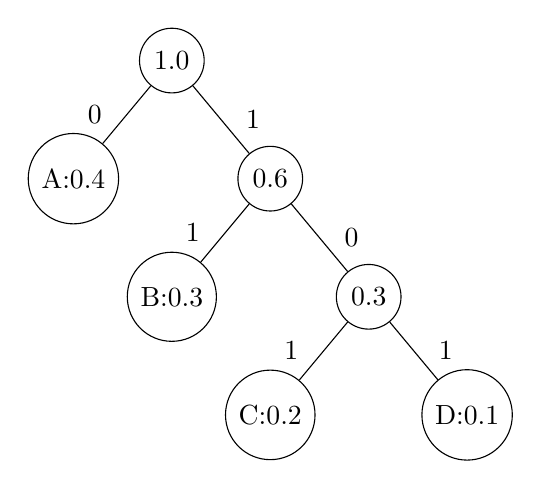
\begin{tikzpicture}[level distance=1.5cm, sibling distance=2.5cm, every node/.style={circle, draw, minimum size=0.8cm}]
    \node {1.0}
        child {node {A:0.4} edge from parent node[left, draw=none] {0}}
        child {node {0.6}
            child {node {B:0.3} edge from parent node[left, draw=none] {1}}
            child {node {0.3}
                child {node {C:0.2} edge from parent node[left, draw=none] {1}}
                child {node {D:0.1} edge from parent node[right, draw=none] {1}}
            edge from parent node[right, draw=none] {0}}
        edge from parent node[right, draw=none] {1}};
\end{tikzpicture}
\captionof{figure}{Huffman Tree}
\end{center}

\begin{center}
\captionof{table}{Huffman Codes}
\begin{tabulary}{\linewidth}{|C|C|C|}
\hline
\textbf{Character} & \textbf{Probability} & \textbf{Code} \\ \hline
A & 0.4 & 0 \\ \hline
B & 0.3 & 10 \\ \hline
C & 0.2 & 110 \\ \hline
D & 0.1 & 111 \\ \hline
\end{tabulary}
\end{center}

\begin{itemize}
    \item \keyword{Average code length}: $0.4 \times 1 + 0.3 \times 2 + 0.2 \times 3 + 0.1 \times 3 = 1.9$ bits
    \item \keyword{Compression achieved}: Reduces average bits per character
    \item \keyword{Prefix property}: No code is prefix of another
\end{itemize}
\end{solutionbox}

\begin{mnemonicbox}
\mnemonic{Huffman Minimum Average Length - HMAL}
\end{mnemonicbox}

\questionmarks{3(a OR)}{3}{State the significance of probability and entropy in communication}

\begin{solutionbox}
\begin{center}
\captionof{table}{Significance of Concepts}
\begin{tabulary}{\linewidth}{|L|L|}
\hline
\textbf{Concept} & \textbf{Significance} \\ \hline
\textbf{Probability} & Measures likelihood of information occurrence \\ \hline
\textbf{Entropy} & Measures average information content \\ \hline
\textbf{Maximum Entropy} & Occurs with equal probability events \\ \hline
\end{tabulary}
\end{center}

\begin{itemize}
    \item \keyword{Information content}: $I = \log_2(1/P)$ bits
    \item \keyword{Entropy formula}: $H = -\sum P(x) \log_2 P(x)$
    \item \keyword{Channel design}: Helps optimize communication systems
    \item \keyword{Coding efficiency}: Guides source coding design
\end{itemize}
\end{solutionbox}

\begin{mnemonicbox}
\mnemonic{Probability Entropy Information - PEI communication}
\end{mnemonicbox}

\questionmarks{3(b OR)}{4}{Explain simplex, half duplex and full duplex data transmission mode}

\begin{solutionbox}
\begin{center}
\captionof{table}{Transmission Modes}
\begin{tabulary}{\linewidth}{|L|L|L|L|}
\hline
\textbf{Mode} & \textbf{Direction} & \textbf{Example} & \textbf{Flow} \\ \hline
\textbf{Simplex} & One-way only & Radio broadcast & A $\rightarrow$ B \\ \hline
\textbf{Half Duplex} & Both ways, not simultaneous & Walkie-talkie & A $\leftrightarrow$ B \\ \hline
\textbf{Full Duplex} & Both ways, simultaneous & Telephone & A $\rightleftarrows$ B \\ \hline
\end{tabulary}
\end{center}

\begin{itemize}
    \item \keyword{Simplex}: Unidirectional communication
    \item \keyword{Half duplex}: Bidirectional but alternate
    \item \keyword{Full duplex}: Simultaneous bidirectional
    \item \keyword{Bandwidth requirement}: Full duplex needs twice the bandwidth
\end{itemize}
\end{solutionbox}

\begin{mnemonicbox}
\mnemonic{Simple Half Full - SHF transmission modes}
\end{mnemonicbox}

\questionmarks{3(c OR)}{7}{Explain Shannon Fano coding with help of suitable example}

\begin{solutionbox}
\textbf{Example: Characters A, B, C, D with probabilities 0.4, 0.3, 0.2, 0.1}

\textbf{Shannon-Fano Algorithm Steps:}
\begin{enumerate}
    \item \textbf{Step 1}: Arrange in descending order (A: 0.4, B: 0.3, C: 0.2, D: 0.1)
    \item \textbf{Step 2}: Divide into two groups
    \begin{itemize}
        \item Group 1: A(0.4) $\rightarrow$ Code starts with 0
        \item Group 2: B(0.3), C(0.2), D(0.1) $\rightarrow$ Code starts with 1
    \end{itemize}
    \item \textbf{Step 3}: Subdivide Group 2
    \begin{itemize}
        \item B(0.3) $\rightarrow$ Code: 10
        \item C(0.2), D(0.1) $\rightarrow$ Code starts with 11
    \end{itemize}
    \item \textbf{Step 4}: Final subdivision
    \begin{itemize}
        \item C(0.2) $\rightarrow$ Code: 110
        \item D(0.1) $\rightarrow$ Code: 111
    \end{itemize}
\end{enumerate}

\begin{center}
\captionof{table}{Shannon-Fano Codes}
\begin{tabulary}{\linewidth}{|C|C|C|}
\hline
\textbf{Character} & \textbf{Probability} & \textbf{Code} \\ \hline
A & 0.4 & 0 \\ \hline
B & 0.3 & 10 \\ \hline
C & 0.2 & 110 \\ \hline
D & 0.1 & 111 \\ \hline
\end{tabulary}
\end{center}

\begin{itemize}
    \item \keyword{Average length}: Same as Huffman (1.9 bits)
    \item \keyword{Top-down approach}: Divides from root to leaves
    \item \keyword{Not always optimal}: Huffman is generally better
\end{itemize}
\end{solutionbox}

\begin{mnemonicbox}
\mnemonic{Shannon Fano Top-Down - SFTD coding}
\end{mnemonicbox}

\questionmarks{4(a)}{3}{Describe Ethical and Privacy Considerations in Data Communication}

\begin{solutionbox}
\begin{center}
\captionof{table}{Ethics and Privacy}
\begin{tabulary}{\linewidth}{|L|L|}
\hline
\textbf{Aspect} & \textbf{Consideration} \\ \hline
\textbf{Data Privacy} & User consent, data protection \\ \hline
\textbf{Security} & Encryption, access control \\ \hline
\textbf{Transparency} & Clear data usage policies \\ \hline
\end{tabulary}
\end{center}

\begin{itemize}
    \item \keyword{Privacy rights}: Users control over personal data
    \item \keyword{Ethical use}: Responsible data handling practices
    \item \keyword{Legal compliance}: Following data protection laws
    \item \keyword{Security measures}: Protecting against unauthorized access
\end{itemize}
\end{solutionbox}

\begin{mnemonicbox}
\mnemonic{Privacy Security Transparency - PST ethics}
\end{mnemonicbox}

\questionmarks{4(b)}{4}{Explain RS 232 standard with pin diagram}

\begin{solutionbox}
\begin{center}
\captionof{table}{RS-232 Pin Configuration (DB-9)}
\begin{tabulary}{\linewidth}{|C|C|L|}
\hline
\textbf{Pin} & \textbf{Signal} & \textbf{Function} \\ \hline
1 & DCD & Data Carrier Detect \\ \hline
2 & RXD & Receive Data \\ \hline
3 & TXD & Transmit Data \\ \hline
4 & DTR & Data Terminal Ready \\ \hline
5 & GND & Ground \\ \hline
6 & DSR & Data Set Ready \\ \hline
7 & RTS & Request To Send \\ \hline
8 & CTS & Clear To Send \\ \hline
9 & RI & Ring Indicator \\ \hline
\end{tabulary}
\end{center}

\begin{itemize}
    \item \keyword{Voltage levels}: +3V to +25V for `0', -3V to -25V for `1'
    \item \keyword{Maximum distance}: 50 feet at 19.2 kbps
    \item \keyword{Applications}: Serial communication between computers and modems
\end{itemize}
\end{solutionbox}

\begin{mnemonicbox}
\mnemonic{RS-232 Nine pins Serial - RNS communication}
\end{mnemonicbox}

\questionmarks{4(c)}{7}{Explain Hamming code with help of suitable example}

\begin{solutionbox}
\textbf{Example: 4-bit data 1011}

\textbf{Hamming Code Construction:}
\begin{center}
\captionof{table}{Hamming Code Bits}
\begin{tabulary}{\linewidth}{|L|C|C|C|C|C|C|C|}
\hline
\textbf{Position} & 1 & 2 & 3 & 4 & 5 & 6 & 7 \\ \hline
\textbf{Type} & P1 & P2 & D1 & P4 & D2 & D3 & D4 \\ \hline
\textbf{Value} & 0 & 1 & 1 & 0 & 0 & 1 & 1 \\ \hline
\end{tabulary}
\end{center}

\begin{itemize}
    \item \keyword{P1} (positions 1,3,5,7): P1 $\oplus$ 1 $\oplus$ 0 $\oplus$ 1 = 0, so P1 = 0
    \item \keyword{P2} (positions 2,3,6,7): P2 $\oplus$ 1 $\oplus$ 1 $\oplus$ 1 = 1, so P2 = 1
    \item \keyword{P4} (positions 4,5,6,7): P4 $\oplus$ 0 $\oplus$ 1 $\oplus$ 1 = 0, so P4 = 0
\end{itemize}

\textbf{Final Hamming Code: 0110111}

\textbf{Error Detection:}
\begin{itemize}
    \item Calculate syndrome $S = S_4S_2S_1$
    \item If $S = 000$, no error
    \item If $S \neq 000$, error at position indicated by S
\end{itemize}

\begin{itemize}
    \item \keyword{Single error correction}: Can correct one-bit errors
    \item \keyword{Double error detection}: Can detect two-bit errors
    \item \keyword{Systematic approach}: Organized parity bit placement
\end{itemize}
\end{solutionbox}

\begin{mnemonicbox}
\mnemonic{Hamming Single Error Correction - HSEC}
\end{mnemonicbox}

\questionmarks{4(a OR)}{3}{Define Edge Computing and explain feature of it}

\begin{solutionbox}
\begin{center}
\captionof{table}{Edge Computing Features}
\begin{tabulary}{\linewidth}{|L|L|}
\hline
\textbf{Feature} & \textbf{Description} \\ \hline
\textbf{Low Latency} & Processing near data source \\ \hline
\textbf{Bandwidth Saving} & Reduces network traffic \\ \hline
\textbf{Real-time Processing} & Immediate data analysis \\ \hline
\end{tabulary}
\end{center}

\begin{itemize}
    \item \keyword{Definition}: Computing at network edge, close to data sources
    \item \keyword{Reduced latency}: Faster response times
    \item \keyword{Distributed processing}: Reduces central server load
    \item \keyword{Applications}: IoT, autonomous vehicles, smart cities
\end{itemize}
\end{solutionbox}

\begin{mnemonicbox}
\mnemonic{Edge Low-latency Real-time - ELR computing}
\end{mnemonicbox}

\questionmarks{4(b OR)}{4}{Explain needs of multimedia processing for communication and various file formats of different data}

\begin{solutionbox}
\begin{center}
\captionof{table}{Multimedia File Formats}
\begin{tabulary}{\linewidth}{|L|L|L|}
\hline
\textbf{Data Type} & \textbf{Formats} & \textbf{Characteristics} \\ \hline
\textbf{Audio} & MP3, WAV, AAC & Compressed/Uncompressed \\ \hline
\textbf{Video} & MP4, AVI, MOV & Different codecs \\ \hline
\textbf{Image} & JPEG, PNG, GIF & Lossy/Lossless compression \\ \hline
\textbf{Text} & TXT, PDF, DOC & Various encodings \\ \hline
\end{tabulary}
\end{center}

\begin{itemize}
    \item \keyword{Processing needs}: Compression, format conversion, quality optimization
    \item \keyword{Bandwidth optimization}: Reducing file sizes for transmission
    \item \keyword{Quality preservation}: Maintaining acceptable quality levels
    \item \keyword{Compatibility}: Supporting multiple devices and platforms
\end{itemize}
\end{solutionbox}

\begin{mnemonicbox}
\mnemonic{Audio Video Image Text - AVIT multimedia}
\end{mnemonicbox}

\questionmarks{4(c OR)}{7}{Explain different Line coding with help of waveform}

\begin{solutionbox}
\textbf{Line Coding Waveforms for data 1011:}
\begin{center}
\begin{tikzpicture}[x=1cm,y=0.6cm]
    % Data
    \node at (-2, 1) {Data:};
    \foreach \x/\val in {0/1, 1/0, 2/1, 3/1} {
        \draw (\x,0) -- (\x,\val) -- (\x+1,\val) -- (\x+1,0); 
        \node at (\x+0.5, 1.5) {\val};
    }
    
    % NRZ-L
    \node at (-2, -1.5) {NRZ-L:};
    \foreach \x/\val in {0/1, 1/0, 2/1, 3/1} {
        \ifnum\val=1
            \draw (\x,-1) -- (\x+1,-1); % High
        \else
            \draw (\x,-2) -- (\x+1,-2); % Low
        \fi
        \ifnum\x>0 \draw (\x,-1) -- (\x,-2); \fi % Transition
        \ifnum\x=0 \ifnum\val=1 \draw (0,-2) -- (0,-1); \fi \fi
    }
    
    % NRZ-I
    \node at (-2, -4) {NRZ-I:};
    \draw (0,-3) -- (1,-3); % 1 -> toggle to low (assuming start high)
    \draw (1,-3) -- (2,-3); % 0 -> same
    \draw (2,-3) -- (3,-2); % 1 -> toggle to high
    \draw (3,-2) -- (4,-3); % 1 -> toggle to low
    % Vertical lines
    \draw (2,-3) -- (2,-2);
    \draw (3,-2) -- (3,-3);
    
    % RZ
    \node at (-2, -6.5) {RZ:};
    \foreach \x/\val in {0/1, 1/0, 2/1, 3/1} {
        \ifnum\val=1
            \draw (\x,-5.5) -- (\x+0.5,-5.5) -- (\x+0.5,-6.5) -- (\x+1,-6.5);
            \draw (\x,-6.5) -- (\x,-5.5);
        \else
            \draw (\x,-6.5) -- (\x+1,-6.5);
        \fi
    }
    
    % Manchester
    \node at (-2, -9) {Manchester:};
    \foreach \x/\val in {0/1, 1/0, 2/1, 3/1} {
        \ifnum\val=1
            \draw (\x,-8) -- (\x+0.5,-8) -- (\x+0.5,-9) -- (\x+1,-9);
            \ifnum\x>0 \draw (\x,-9) -- (\x,-8); \fi
        \else
            \draw (\x,-9) -- (\x+0.5,-9) -- (\x+0.5,-8) -- (\x+1,-8);
             \ifnum\x>0 \draw (\x,-9) -- (\x,-8); \fi
        \fi
    }
\end{tikzpicture}
\captionof{figure}{Line Coding Waveforms}
\end{center}

\begin{center}
\captionof{table}{Line Coding Comparison}
\begin{tabulary}{\linewidth}{|L|L|L|L|}
\hline
\textbf{Code Type} & \textbf{Bandwidth} & \textbf{DC Component} & \textbf{Synchronization} \\ \hline
\textbf{NRZ-L} & Low & Present & Poor \\ \hline
\textbf{NRZ-I} & Low & Present & Poor \\ \hline
\textbf{RZ} & High & Present & Good \\ \hline
\textbf{Manchester} & High & Absent & Excellent \\ \hline
\end{tabulary}
\end{center}

\begin{itemize}
    \item \keyword{NRZ}: Non-Return-to-Zero, simple but has DC component
    \item \keyword{RZ}: Return-to-Zero, better synchronization
    \item \keyword{Manchester}: Self-synchronizing, no DC component
    \item \keyword{Selection criteria}: Bandwidth, synchronization, complexity
\end{itemize}
\end{solutionbox}

\begin{mnemonicbox}
\mnemonic{NRZ RZ Manchester - NRM line codes}
\end{mnemonicbox}

\questionmarks{5(a)}{3}{Explain concept of spread spectrum technology}

\begin{solutionbox}
\begin{center}
\captionof{table}{Spread Spectrum Characteristics}
\begin{tabulary}{\linewidth}{|L|L|}
\hline
\textbf{Parameter} & \textbf{Description} \\ \hline
\textbf{Bandwidth Spreading} & Signal spread over wide frequency \\ \hline
\textbf{Low Power Density} & Power distributed across spectrum \\ \hline
\textbf{Interference Resistance} & Resistant to jamming \\ \hline
\end{tabulary}
\end{center}

\begin{itemize}
    \item \keyword{Principle}: Spreads signal over much wider bandwidth than required
    \item \keyword{Techniques}: Direct Sequence (DS-SS), Frequency Hopping (FH-SS)
    \item \keyword{Advantages}: Security, interference resistance, multiple access
    \item \keyword{Applications}: GPS, CDMA, WiFi, Bluetooth
\end{itemize}
\end{solutionbox}

\begin{mnemonicbox}
\mnemonic{Spread Spectrum Security - SSS technology}
\end{mnemonicbox}

\questionmarks{5(b)}{4}{Explain block diagram of satellite communication}

\begin{solutionbox}
\begin{center}
\begin{tikzpicture}[node distance=1.5cm, auto]
    \node [gtu block] (sat) {Satellite Transponder};
    \node [gtu block, below left=2cm of sat] (es1) {Earth Station 1};
    \node [gtu block, below right=2cm of sat] (es2) {Earth Station 2};
    \node [left=0.5cm of sat] (ant1) {Antenna};
    \node [right=0.5cm of sat] (ant2) {Antenna};
    
    \draw [gtu arrow] (es1) -- node[sloped, above] {Uplink} (sat);
    \draw [gtu arrow] (sat) -- node[sloped, above] {Downlink} (es2);
    \draw [dotted] (ant1) -- (sat);
    \draw [dotted] (ant2) -- (sat);
\end{tikzpicture}
\captionof{figure}{Satellite Communication}
\end{center}

\begin{center}
\captionof{table}{Satellite Communication Components}
\begin{tabulary}{\linewidth}{|L|L|}
\hline
\textbf{Component} & \textbf{Function} \\ \hline
\textbf{Earth Station} & Ground-based transmit/receive \\ \hline
\textbf{Uplink} & Earth to satellite transmission \\ \hline
\textbf{Transponder} & Satellite receiver-transmitter \\ \hline
\textbf{Downlink} & Satellite to earth transmission \\ \hline
\end{tabulary}
\end{center}

\begin{itemize}
    \item \keyword{Frequency bands}: C-band, Ku-band, Ka-band
    \item \keyword{Coverage area}: Large geographical coverage
    \item \keyword{Applications}: Broadcasting, telephony, internet
    \item \keyword{Advantages}: Wide coverage, long-distance communication
\end{itemize}
\end{solutionbox}

\begin{mnemonicbox}
\mnemonic{Earth Uplink Transponder Downlink - EUTD satellite}
\end{mnemonicbox}

\questionmarks{5(c)}{7}{Demonstrate model of Multimedia Communications and elements of Multimedia system}

\begin{solutionbox}
\textbf{Multimedia Communication Model:}
\begin{center}
\begin{tikzpicture}[node distance=1.2cm, auto]
    \node [gtu block] (enc) {Encoder};
    \node [gtu block, right=1cm of enc] (mux) {Multiplexer};
    \node [gtu block, right=1cm of mux] (net) {Network};
    \node [gtu block, right=1cm of net] (demux) {Demultiplexer};
    \node [gtu block, right=1cm of demux] (dec) {Decoder};
    \node [gtu block, right=1cm of dec] (dest) {Destination};
    
    \node [left=1cm of enc] (source) {Source Inputs};
    \node [above=0.2cm of source] (aud) {Audio};
    \node [below=0.2cm of source] (vid) {Video};
    \node [above=0.6cm of source] (txt) {Text};
    \node [below=0.6cm of source] (gfx) {Graphics};
    
    \draw [gtu arrow] (aud) -- (enc);
    \draw [gtu arrow] (vid) -- (enc);
    \draw [gtu arrow] (txt) -- (enc);
    \draw [gtu arrow] (gfx) -- (enc);
    
    \draw [gtu arrow] (enc) -- (mux);
    \draw [gtu arrow] (mux) -- (net);
    \draw [gtu arrow] (net) -- (demux);
    \draw [gtu arrow] (demux) -- (dec);
    \draw [gtu arrow] (dec) -- (dest);
\end{tikzpicture}
\captionof{figure}{Multimedia Communication Model}
\end{center}

\begin{center}
\captionof{table}{Multimedia System Elements}
\begin{tabulary}{\linewidth}{|L|L|L|}
\hline
\textbf{Element} & \textbf{Function} & \textbf{Examples} \\ \hline
\textbf{Capture} & Input multimedia data & Camera, microphone \\ \hline
\textbf{Storage} & Store multimedia files & Hard disk, memory \\ \hline
\textbf{Processing} & Edit and manipulate & Video editing software \\ \hline
\textbf{Communication} & Transmit multimedia & Networks, internet \\ \hline
\textbf{Presentation} & Display multimedia & Monitor, speakers \\ \hline
\end{tabulary}
\end{center}

\begin{itemize}
    \item \keyword{Synchronization}: Audio-video synchronization critical
    \item \keyword{Compression}: Reduces bandwidth requirements
    \item \keyword{Quality of Service}: Maintains acceptable quality
    \item \keyword{Real-time constraints}: Time-sensitive data delivery
\end{itemize}
\end{solutionbox}

\begin{mnemonicbox}
\mnemonic{Capture Store Process Communicate Present - CSPCP multimedia}
\end{mnemonicbox}

\questionmarks{5(a OR)}{3}{Explain importance of Block chain in Communication Security}

\begin{solutionbox}
\begin{center}
\captionof{table}{Blockchain Security Features}
\begin{tabulary}{\linewidth}{|L|L|}
\hline
\textbf{Feature} & \textbf{Benefit} \\ \hline
\textbf{Decentralization} & No single point of failure \\ \hline
\textbf{Immutability} & Cannot alter past records \\ \hline
\textbf{Transparency} & All transactions visible \\ \hline
\end{tabulary}
\end{center}

\begin{itemize}
    \item \keyword{Cryptographic security}: Hash functions and digital signatures
    \item \keyword{Distributed ledger}: Multiple copies prevent tampering
    \item \keyword{Smart contracts}: Automated security protocols
    \item \keyword{Applications}: Secure messaging, identity verification
\end{itemize}
\end{solutionbox}

\begin{mnemonicbox}
\mnemonic{Blockchain Distributed Immutable - BDI security}
\end{mnemonicbox}

\questionmarks{5(b OR)}{4}{Explain important elements, features and advantages of 5G technology}

\begin{solutionbox}
\begin{center}
\captionof{table}{5G Specifications}
\begin{tabulary}{\linewidth}{|L|L|}
\hline
\textbf{Element} & \textbf{Specification} \\ \hline
\textbf{Speed} & Up to 10 Gbps \\ \hline
\textbf{Latency} & Less than 1 ms \\ \hline
\textbf{Connections} & 1 million devices per km\textsuperscript{2} \\ \hline
\textbf{Reliability} & 99.999\% availability \\ \hline
\end{tabulary}
\end{center}

\textbf{Key Features:}
\begin{itemize}
    \item \keyword{Enhanced Mobile Broadband}: Ultra-high-speed internet
    \item \keyword{Ultra-Reliable Low Latency}: Critical applications
    \item \keyword{Massive Machine Communication}: IoT connectivity
    \item \keyword{Network Slicing}: Customized network services
\end{itemize}

\textbf{Advantages:}
\begin{itemize}
    \item \keyword{Higher capacity}: More simultaneous users
    \item \keyword{Energy efficiency}: Better battery life for devices
    \item \keyword{New applications}: AR/VR, autonomous vehicles
\end{itemize}
\end{solutionbox}

\begin{mnemonicbox}
\mnemonic{5G Speed Latency Connections - SLC features}
\end{mnemonicbox}

\questionmarks{5(c OR)}{7}{Compare RS 232, RS 422 and RS 485 standard}

\begin{solutionbox}
\begin{center}
\captionof{table}{RS Standards Comparison}
\begin{tabulary}{\linewidth}{|L|L|L|L|}
\hline
\textbf{Parameter} & \textbf{RS-232} & \textbf{RS-422} & \textbf{RS-485} \\ \hline
\textbf{Mode} & Single-ended & Differential & Differential \\ \hline
\textbf{Max Distance} & 50 feet & 4000 feet & 4000 feet \\ \hline
\textbf{Max Speed} & 20 kbps & 10 Mbps & 10 Mbps \\ \hline
\textbf{Drivers} & 1 & 1 & 32 \\ \hline
\textbf{Receivers} & 1 & 10 & 32 \\ \hline
\textbf{Topology} & Pt-to-Pt & Pt-to-Multi & Multipoint \\ \hline
\end{tabulary}
\end{center}

\begin{center}
\captionof{table}{Voltage Levels}
\begin{tabulary}{\linewidth}{|L|L|L|}
\hline
\textbf{Standard} & \textbf{Logic 1} & \textbf{Logic 0} \\ \hline
\textbf{RS-232} & -3V to -25V & +3V to +25V \\ \hline
\textbf{RS-422} & Diff $< -200$mV & Diff $> +200$mV \\ \hline
\textbf{RS-485} & Diff $< -200$mV & Diff $> +200$mV \\ \hline
\end{tabulary}
\end{center}

\begin{itemize}
    \item \keyword{Applications}: RS-232 (PC serial), RS-422 (Industrial), RS-485 (Building automation)
    \item \keyword{Noise immunity}: Differential signaling in RS-422/485 better than RS-232
    \item \keyword{Distance capability}: RS-422/485 much longer than RS-232
    \item \keyword{Cost}: RS-232 cheapest, RS-485 most complex
\end{itemize}
\end{solutionbox}

\begin{mnemonicbox}
\mnemonic{RS-232 Simple, RS-422 Long, RS-485 Multi - SLM standards}
\end{mnemonicbox}

\end{document}
